%\chapter{Modelling Phonemic Streams using Transformer Language Models}\label{chapter:modelling}
\chapter{Establishing the feasibility of Phoneme LMs}\label{chapter:modelling}

\section{Abstract}

Language models are typically trained on large corpora of text in their default orthographic form. However, this is not the only option; representing data as streams of phonemes can offer unique advantages, from deeper insights into phonological language acquisition to improved performance on sound-based tasks. The challenge lies in evaluating the impact of phoneme-based training, as most benchmarks are also orthographic. To address this, we develop a pipeline to convert text datasets into a continuous stream of phonemes. We apply this pipeline to the 100-million-word pre-training dataset from the BabyLM challenge, as well as to standard language and grammatical benchmarks, enabling us to pre-train and evaluate a model using phonemic input representations. Our results show that while phoneme-based training slightly reduces performance on traditional language understanding tasks, it offers valuable analytical and practical benefits. 

%Possible alternate version:
%Language models are typically trained on large corpora of text in their default orthographic form. However, this is not the only option; representing data as streams of phonemes can offer unique advantages, from deeper insights into phonological language acquisition to improved performance on sound-based tasks. The challenge lies in evaluating the impact of phoneme-based training, as most benchmarks are also orthographic. To address this, we use a grapheme-to-phoneme tool to convert the BabyLM dataset and standard language and grammatical benchmarks into continuous streams of phonemes and use these to pre-train and evaluate a language model based on GPT-2. Our results show that while phoneme-based training slightly reduces performance on traditional language understanding tasks, it offers valuable analytical and practical benefits.% and useful insights into the consequences of choosing particular input representation. 

\section{Introduction}

% 1. When neural networks were first invented, they were fed continuous streams of phonemic or graphemic characters and people were amazed by their ability to learn the statistical rules of language. 30 years later, language models have grown considerably, and the standard input representation has been developed to suit downstream applications.

The use of orthographic text to train neural networks is so commonplace that it is considered the default. This has not always been the case.

When neural networks were first applied to language, models were primarily trained on continuous streams of phonemes or graphemes, rather than orthographic text with its written artefacts. These early neural models demonstrated a striking ability to acquire phonology, syntax and semantics \citep{elman-1990-finding, seidenberg-1989-word-recognition, prince-1997-optimality}. As technology scaled, subword representations became the dominant representation, offering key advantages such as reducing computation costs and better capturing out-of-vocabulary items \citep{sennrich-etal-2016-bpe}. Written text became favored over speech transcriptions due to matching the domain of downstream tasks and due to the abundance of diverse texts available through web-scraping \citep{bansal-2022-datascaling}. Today, ``large language models'' (LLMs) all use subword-based text inputs and perform impressively on a variety of language understanding tasks \citep{zellers-etal-2019-hellaswag, hendrycks-2020-mmlu, suzgun-2023-Big-Bench}.

\begin{figure}[t]
    \centering
    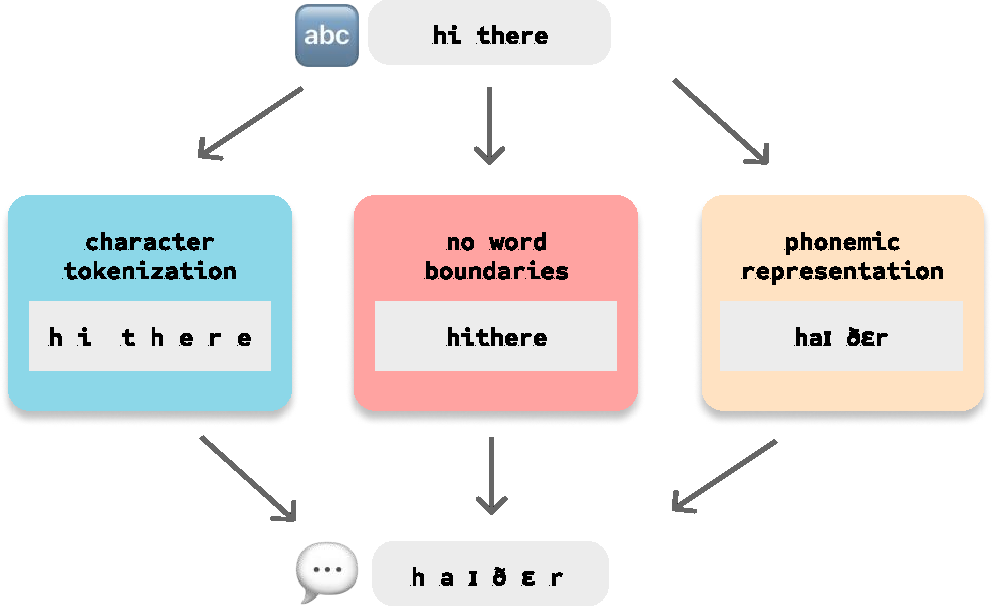
\includegraphics[width=\linewidth]{14Modelling/example.pdf}
    \caption{An illustration of all three adjustments that we make to convert text input to continuous streams of phonemes.}
    \label{fix:14-example}
    \vspace{-6mm}
\end{figure}

% 2. SOTA models use BPE and orthographic as default, and many probing studies followed in order to try to understand how these models learn language. However, written text was still the default, and so analysing phonological capabilities is hard.

%The success of these models on downstream tasks has motivated researchers to examine how LLMs learn grammatical generalizations and represent language internally \citep{hewitt-manning-2019-structural, hu-etal-2020-systematic, manning-2020-emergent}. However, the orthographic nature of training data has made it challenging to analyze the phonological capabilities of these LLMs. 

\zeb{Moved to background} The success of these models on downstream tasks has motivated researchers to examine the internal representations of LLMs and analyze their ability to learn grammatical generalizations \citep{hewitt-manning-2019-structural, hu-etal-2020-systematic, manning-2020-emergent}. However, their phonological capabilities remain understudied due to the orthographic nature of training data.

%[OLD] These emergent capabilities of LMs are largely attributed to the trillions of web-scraped text tokens that they are pre-trained on \citep{touvron-2023-llama, hoffmann-2022-chinchilla}. 

% 3. The use of phonemes as an underlying input representation has analytical and practical benefits. Probing studies who want to research the statistical properties of phoememe strings, acquisition studies who want to emulate the acquisition of words or grammar rules, as well as practical studies who want units to have auditory representations. 

An alternative input representation for text-based language models is to use phonemes rather than graphemes, corresponding to how words are pronounced, rather than how they are written. The use of phonemes, such as those described by the International Phonetic Alphabet (IPA), as an underlying input representation, presents the following analytical and practical benefits over an orthographic representation that is the modern-day default.

\paragraph{Analytical:} A phoneme-based representation is useful when using language models to study the distributional properties of phonemes \citep{mayer-2020-phonology-distribution} and phonological systems of languages more broadly \citep{eden-2018-phonological-distance}. Many language acquisition studies prefer using phonemes as a representation that more closely represents the human learning environment, which facilitates statistical learning experiments ranging from word segmentation \citep{Coltekin2017}, to past-tense formation \citep{kirov-2018-recurrent}, and broader lexico-syntactic knowledge \citep{lavechin}.

\paragraph{Practical:} IPA-encoded text has been found to be beneficial for a variety of NLP tasks including lyric generation \citep{ding-2024-songcomposer}, text-to-speech \citep{sundararaman-2021-phonemebert, li-2023-phoneme-level-bert} and low-resource language modeling \citep{leong-whitenack-2022-phone}. Phonemes also benefit multi-lingual language modeling by establishing a universal representation shared between languages \citep{feng-2023-language-universal-phonetic, zhu-etal-2024-taste}. 

% There are also benefits to using a phonemic representation when it comes to multi-lingual language modeling as orthographic rules vary considerably between languages and previous work has struggled with representing the vocabulary of multiple languages, often disadvantaging low-resource languages as a consequence [cite xlm-r/xlm  papers].

%Phonemes also provide benefits particularly in the context of multi-lingual language modelling. Previous work has struggled with modelling the vocabulary of multiple languages, and has historically resorted to using language-specific tokenization [xlm paper]. one of the issues of using a single vocabulary is that orthographically divergent low-resource languages are disadvanted [xlm-r paper].  and often require the use of specila tokenization approaches such as    Using continuous streams of phonemes provides a universal 

% 4. It is of interest to all of these branches to understand whether the standard transformer architecture now so very popular in NLP is appropriate for an input representation consisting of a continuous stream of individual phonemes. It is also of interest to those to have a quick way of getting data. 

\vspace{.3cm}

Despite the analytical and practical advantages of training language models with phonemes, a key question remains: \emph{Can modern language model architectures encode grammatical knowledge and succeed at language understanding tasks when trained with phoneme-based representations?} 

Answering this question is challenging for two reasons. First, training and evaluation data need to be provided to a model in both a phonemic and graphemic representation. Second, it is non-trivial to select the transformations to convert orthographic text into phonemic representations and to evaluate how these individually affect a model's performance across a wide variety of benchmarks.

%the differences between the standard orthographic and phonemic representations and considering whether any gaps in performance may be due to a single transformation, rather than the entire change.

% 5. We identify three key transformations and provide the tools to phonemize this data and train a model on a large corpus of phonemes. We run a careful ablation of the effects of each of these transformation in isolation and combination. 

In this work, we address these challenges as follows. We first present a method for converting training data and evaluation benchmarks into a unified IPA representation. This enables language models to be trained and evaluated on graphemic and phonemic representations of the same data. We then identify three key transformations which enable us to map from the written representation typically used to train language models to the phonemic representation often used in analytical studies (see \cref{fix:14-example}). Finally, we conduct a careful ablation of the three transformations: we train a language model on the same corpus of 100 million words with all combinations of the three transformations ($2^3$ configurations), evaluating the model's grammatical capabilities and its resulting performance on downstream language understanding tasks. 

% 6. Results and conclusions

We find that large language models are powerful statistical learners capable of learning grammar from a phonemic input representation. Although we observe a decrease in performance on some tasks, the degradation is not as substantial as has been anecdotally suggested by previous studies. Our ablation studies indicate that the impact of each transformation that we use to convert orthographic text to continuous phoneme streams depends on the downstream task; tasks in the BLiMP Supplement set are particularly sensitive to the use of phonemes, while those in GLUE are sensitive to character tokenization. A deeper analysis into these ablations reveals that many evaluation instances rely on information only present in written text (such as punctuation). Finally, we take advantage of the fact that we train models using phonemic streams and evaluate our models for phonological knowledge using the BabySLM benchmark. Our models achieve the best scores on this benchmark to date.%, suggesting that these models have many unexplored benefits. 

%Finally, because the models we train accept phonetic inputs we train the language models usrepresentation can be evaluated for phonological knowledge - we do so and we achieve the best scores on the BabySLM corpus to date. Our novel use of the byte-pair encoding (BPE) algorithm on text with spaces removed may also lead to interesting acquisition studies relating to word segmentation and lexicon learning. 

% We discuss the limitations of our transcription method and discuss the use of raw audio as an alternative input representation. Finally, we present the advantages of this input representation for multi-lingual and low-resource applications and encourage further work in phoneme-based language modeling. 


\section{tmpintro}

We identify three key transformations that bring us from the standard input representation used by language models to this alternative \textbf{phoneme stream} representation:

% \begin{itemize}
%     \item Using a character-based tokenization instead of using subwords.
%     \item Removing word boundaries from the input.
%     \item Using phonemic transcriptions instead of written text.
% \end{itemize}

\begin{itemize}
\setlength\itemsep{0.1em}
    \item \characterhighlight{Character tokenization} Treating each phoneme or grapheme as a token, rather than using subwords.
    \item \spacehighlight{Word boundary removal} Removing whitespace or other word boundary cues from the input.
    \item \phonemehighlight{Phonemic transcription} Converting words to a phonemic representation. 
\end{itemize}

\noindent
Each transformation can be made independently or in combination, as illustrated in \cref{fix:14-example}. %By implementing every possible combination, we can identify the impact of each transformation on language learning by LLMs. 
% We can also create novel representations of the input which may not have been considered (such as learning subword units from text stripped of word boundaries). 
% The three input transformations have mostly been studied separately. 


\section{Phoneme Stream Pipeline}
\label{sec:14-pipeline}

To convert the data to a phonemic representation, we developed the \textbf{Corpus Phonemizer} tool:\footnote{\url{https://github.com/codebyzeb/Corpus-Phonemizer}}\zeb{fix this} a library to convert various corpora across many different languages to a unified phonemic representation in IPA, prepare them as Huggingface datasets and subsequently train Huggingface tokenizers.

\subsection{Dataset Phonemization}

Our toolkit leverages the \texttt{phonemizer} package \citep{Bernard2021} with the \texttt{espeak-ng} backend\footnote{\url{https://github.com/espeak-ng/espeak-ng}} which uses a combination of a pronunciation dictionary and pronunciation rules to convert orthographic transcriptions to IPA. We select the American English accent (\texttt{en-US}) for a consistent pronunciation. 

The tool outputs phonemes separated by spaces.\footnote{It is common practice to separate phonemes by spaces to make tokenization simple, as some individual phonemes may consist of several symbols, e.g. \textipa{tS} or \textipa{3I}.} For instance, the phonemic representation of ``what a conundrum!'' is:

\vspace{-2mm}
\begin{center}
\texttt{\textipa{w 2 t} \textvisiblespace~\textipa{2} \textvisiblespace~\textipa{
k @ n 2 n d \*r @ m} \textvisiblespace~}
\end{center}
\vspace{-1mm}

\noindent
One limitation of our phonemization tool is that `a' is not reduced to the shwah, `\textipa{@}', as it would be in continuous speech. We discuss the limitations of this phonemization process in \cref{sec:14-phonemeslimitations}. Crucially, we lose punctuation marks, as they are an artefact of orthographic text and equivalent information in speech would be conveyed through prosody, stress, or non-linguistic signals such as gestures, none of which are included in this simple phonemic format. This has potential consequences for downstream tasks that rely on such markers, as discussed in \cref{sec:14-punctuation}.

\begin{table*}[t]
    \centering
    \small
    \addtolength{\tabcolsep}{-0.2em}
    \begin{tabular}{l||ccc|c|c||ccccc}
       Model & \rotatebox[origin=l]{90}{\characterhighlight{Character tokenization}} & \rotatebox[origin=l]{90}{\spacehighlight{Word boundary removal}} & \rotatebox[origin=l]{90}{\phonemehighlight{Phonemic transcription}} & \rotatebox[origin=l]{90}{Vocabulary Size} & Example Tokenization & \rotatebox[origin=l]{90}{BLiMP Filtered} & \rotatebox[origin=l]{90}{BLiMP Supplement} & \rotatebox[origin=l]{90}{GLUE} & \rotatebox[origin=l]{90}{BabySLM (Syntactic)} & \rotatebox[origin=l]{90}{BabySLM ( Lexical)} \\
       \midrule
        Baby Llama & \xmark & \xmark & \xmark & 16,000 & ~\mybox{\textvisiblespace what} ~\mybox{\textvisiblespace a} ~\mybox{\textvisiblespace con} ~\mybox{und} ~\mybox{rum} ~\mybox{\textvisiblespace !} & 73.1 & 60.6 & 69.0 &  94.0 & - \\
        LTG-BERT & \xmark & \xmark & \xmark & 16,000 & ~\mybox{\textvisiblespace what} ~\mybox{\textvisiblespace a} ~\mybox{\textvisiblespace con} ~\mybox{und} ~\mybox{r} ~\mybox{um} ~\mybox{\textvisiblespace !} & 69.3 & 66.5 & 68.4 & 75.8 & - \\
        \midrule
         & \xmark & \xmark & \xmark & 16,000 & ~\mybox{\textvisiblespace what} ~\mybox{\textvisiblespace a} ~\mybox{\textvisiblespace con} ~\mybox{und}  ~\mybox{rum} ~\mybox{\textvisiblespace!} & \textbf{77.8} & \textbf{69.4} & \textbf{71.6} & 92.8 & - \\
         & \xmark & \spacehighlight{\cmark} & \xmark & 16,000 & \mybox{what} ~\mybox{acon} ~\mybox{un} ~\mybox{drum} ~\mybox{!} & 73.9 & 64.3 & 68.6 & 73.9 & - \\
         & \xmark & \xmark & \phonemehighlight{\cmark} & 16,000 & ~\mybox{\textvisiblespace \textipa{w2t}} ~\mybox{\textvisiblespace \textipa{2}} ~\mybox{\textvisiblespace \textipa{k@n}} ~\mybox{\textipa{2nd}} ~\mybox{\textipa{\*r@m}} & 74.7 & 59.6 & 68.6 & 85.8 & 67.3 \\
         \multirow{2}{*}{GPT-2} & \xmark & \spacehighlight{\cmark} & \phonemehighlight{\cmark} & 16,000 & ~\mybox{\textipa{w2t}} ~\mybox{\textipa{2k@n}} ~\mybox{\textipa{2nd}} ~\mybox{\textipa{\*r@m}} & 71.7 & 56.7 & 65.5 & 74.7 & 71.2  \\
         & \characterhighlight{\cmark} & \xmark & \xmark & 115 & \mybox{w} ~\mybox{h} ~\mybox{a} ~\mybox{t} ~\mybox{\textvisiblespace } ~\mybox{a} ~\mybox{\textvisiblespace } ~\mybox{c} ~\mybox{o} ~\mybox{n} ~\mybox{u} ~\mybox{n} ~\mybox{d} ~\mybox{r} ~\mybox{u} ~\mybox{m} ~\mybox{\textvisiblespace } ~\mybox{!} & 77.4 & 63.6 & 64.4 & \textbf{94.9} & - \\
         & \characterhighlight{\cmark} & \spacehighlight{\cmark} & \xmark & 114 & \mybox{w} ~\mybox{h} ~\mybox{a} ~\mybox{t} ~\mybox{a} ~\mybox{c} ~\mybox{o} ~\mybox{n} ~\mybox{u} ~\mybox{n} ~\mybox{d} ~\mybox{r} ~\mybox{u} ~\mybox{m} ~\mybox{!} & 75.1 & 64.8 & 64.8 & 88.3 & - \\
         & \characterhighlight{\cmark} & \xmark & \phonemehighlight{\cmark} & 51 & \mybox{w} ~\mybox{\textipa{2}} ~\mybox{\textipa{t}} ~\mybox{\textvisiblespace } ~\mybox{\textipa{2}}  ~\mybox{\textvisiblespace } ~\mybox{\textipa{k}} ~\mybox{\textipa{@}} ~\mybox{\textipa{n}} ~\mybox{\textipa{2}} ~\mybox{n} ~\mybox{d} ~\mybox{\textipa{\*r}} ~\mybox{\textipa{@}} ~\mybox{m} & 74.7 & 58.5 & 65.6 & 90.5 & \textbf{89.6}  \\
         & \characterhighlight{\cmark} & \spacehighlight{\cmark} & \phonemehighlight{\cmark} & 50 & \mybox{w} ~\mybox{\textipa{2}} ~\mybox{\textipa{t}} ~\mybox{\textipa{2}}  ~\mybox{\textipa{k}} ~\mybox{\textipa{@}} ~\mybox{\textipa{n}} ~\mybox{\textipa{2}} ~\mybox{n} ~\mybox{d} ~\mybox{\textipa{\*r}} ~\mybox{\textipa{@}} ~\mybox{m} & 72.5 & 57.6 & 65.4 & 83.9 & 87.8
    \end{tabular}
    \caption{Results for the two BabyLM baseline models and the GPT-2 model trained under all eight conditions. On the left, we compare the effects of each of the three transformations across all eight possible combinations, by tokenizing the example phrase ``what a conundrum!''. The `\textvisiblespace ' character denotes word boundaries. On the right, we report BLiMP, GLUE and BabySLM scores achieved by each model, with the best scores in each column in \textbf{bold}.} %Note that the BabySLM Lexical score can only be computed for models trained with phonemic input.}
    \label{table:results}
    \vspace{-4mm}
\end{table*}

\subsection{Tokenizer Preparation}

Using the phonemic data transcribed by the Corpus Phonemizer tool, our pipeline then implements the three input transformations by preparing different tokenizers:

\begin{itemize}
\setlength\itemsep{0.1em}
    \item \characterhighlight{Character tokenization} We either train the tokenizer using the Byte-Pair Encoding (BPE) algorithm \citep{sennrich-etal-2016-bpe} (\xmark) or create a character-based tokenizer by extracting a vocabulary from the data (\cmark).
    \item \spacehighlight{Word boundary removal} We either train the tokenizer with whitespace included (\xmark) or use the tokenizer's normalizer to strip whitespace (\cmark).  
    \item \phonemehighlight{Phonemic transcription} The tokenizer is either trained on the original orthographic dataset (\xmark), or the phonemized version described above (\cmark).
\end{itemize}

% \vspace{0.7em}
% \noindent\characterhighlight{Character tokenization} We either train the tokenizer using the Byte-Pair Encoding (BPE) algorithm \citep{sennrich-etal-2016-bpe} or create a character-level tokenizer by extracting a vocabulary of graphemes or phonemes from the data.

% \vspace{0.5em}
% \noindent\spacehighlight{Word boundary removal} We either train the tokenizer with whitespace included or use the tokenizer's normalizer to strip whitespace.  

% \vspace{0.5em}
% \noindent\phonemehighlight{Phonemic transcription} The tokenizer is either trained on the original orthographic dataset or the phonemized version described above.
% \vspace{0.7em}

These transformations can be made independently, allowing for all eight combinations of the transformations to be implemented as individual tokenizers. For the combination of BPE and no word boundaries, the whitespace is removed before training, so the model may learn `subwords' that cross word boundaries.

Each tokenizer also adds a dedicated ``utterance boundary'' token \texttt{UTT\_BOUNDARY} to the start of each sentence, representing the pauses between spoken utterances and serving as a dedicated start-of-sentence token. When sentences are collated, it also implicitly acts as an end-of-sentence token, as discussed in \cref{sec:14-endofsentence}.

\section{Experimental Setup}

We evaluate the effect of our proposed input adjustments by training a GPT-2 model \citep{radford-2019-gpt2} using the BabyLM challenge framework \citep{choshen-et-al-2024-callforpapers-babylm2}. The model is trained eight times with each combination of the three input adjustments. Following the \textsc{strict} track of the BabyLM challenge, we train on a provided corpus of 100 million words and evaluate on a series of benchmarks assessing the grammatical knowledge and the downstream capabilities of each model. We additionally evaluate on BabySLM \citep{lavechin} which provides syntactic and lexical scores specifically for speech-based models. Our phonemized dataset, trained models and tokenizers are hosted on Huggingface.\footnote{\url{https://huggingface.co/collections/phonemetransformers/from-babble-to-words-66e068b54765a48ff30273c9}}
%Below, we describe the BabyLM corpus and how we implemented the three proposed input adjustments (\cref{sec:14-input}). We then describe the GPT-2 model and the BabyLM baseline (\cref{sec:14-model}). Finally, we introduce BLiMP, GLUE and BabySLM in \cref{sec:14-evaluation}.

\subsection{Dataset}
\label{sec:14-input}

The BabyLM 2024 pretraining data contains 100 million words sourced from nine different corpora \citep{warstadt-2023-babylm-findings}. Over 50\% of the data consists of transcribed or scripted speech and over 40\% comes from child-directed sources (written or spoken). %While some studies train models from purely child-directed speech, the BabyLM organisers included additional sources to represent overheard language that a child may learn from and to reach the 100 million word target.
We apply minor cleaning operations to the dataset, removing extraneous spaces and formatting anomalies using regular expressions.

\subsection{Tokenizers}
\label{sec:14-tokenizers}

For each of the eight combinations of the three transformations, we train a tokenizer on the `train' portion of the BabyLM dataset.
We compare the output of the eight tokenizers in \cref{table:results}. We used a vocabulary size of 16,000 for the BPE tokenizers to match the vocabulary size used by the two baseline models provided by the BabyLM challenge (described below). 

Note that the vocabulary size for the character-level tokenizers operating on phonemes is less than half the vocabulary size of their orthographic equivalents. This is because the phonemic data only consists of the 47 phonemes produced by the American English accent, but the orthographic data includes numbers, punctuation and other symbols. 

\subsection{Model}
\label{sec:14-model}

Our experiments use the GPT-2 architecture. We train the model using all eight tokenizers (using the phonemized dataset for the phoneme-based tokenizers) for 400k steps, selecting the checkpoint with the lowest perplexity.\footnote{The best checkpoint for five of the eight models was the final checkpoint but a visual inspection of the curve revealed that differences between the final checkpoints were minimal.} See \cref{app:14-implementation_details} for a full description of the chosen model parameters and training procedure.

We also report the results from two baseline models which achieved the highest scores at the 2023 BabyLM challenge. These are Baby Llama, an auto-regressive model, which was trained using knowledge distillation from an ensemble of teachers \citep{timiryasov-tastet-2023-baby} and LTG-BERT, an architectural variation of the standard auto-encoding BERT architecture optimized for small, speech-based corpora \citep{samuel-etal-2023-trained, charpentier-samuel-2023-layers}. Both models use a BPE tokenizer with a vocabulary size of 16,000 and have a similar number of parameters to our model.\footnote{Our GPT-2 model has 85M non-embedding parameters. Baby Llama has 41M and LTG-Bert has 110M.}  

\subsection{Evaluation}
\label{sec:14-evaluation}

We follow the BabyLM Challenge's framework and evaluate on BLiMP \citep{warstadt-etal-2020-blimp-benchmark}, BLiMP Supplement \citep{choshen-et-al-2024-callforpapers-babylm2} and a subset of the (Super)GLUE tasks \citep{wang-etal-2018-glue, wang-etal-2019-superglue}. BLiMP assesses a model's ability to distinguish grammatical sentences from ungrammatical sentences across 67 subtasks covering a range of linguistic phenomena. BLiMP Supplement consists of 5 BLiMP-style tasks covering additional linguistic phenomena not tested by BLiMP. The GLUE suite assesses a language model's language understanding abilities on typical downstream tasks using fine-tuning. 

% CAN PERHAPS ADD THIS AND PUT RESULTS IN APPENDIX: For completion, we also evaluate on EWoK, which assesses the world knowledge capabilities of a model across several key domains and concepts \citep{ivanova2024elements}.

%BLiMP and BLiMP Supplement are zero-shot metrics; no additional training is required, instead the predictions of a model on pairs of `correct' or `incorrect' examples are used to assess a model's grammatical knowledge. GLUE involves fine-tuning a model and using it for a specific downstream task, assessing its utility for language understanding applications.

We also evaluate our models on BabySLM \citep{lavechin}, a benchmark specifically designed for probing speech-based LMs at a \emph{syntactic} level and a \emph{lexical} level. The benchmark was also designed to compare text-based models (those considered here, including both orthographic text and phonemic transcriptions) to speech-based models (which learn directly from audio) by providing parallel text and audio test instances. Finally, the vocabulary items were chosen to be compatible with children’s language experiences, aiming to better reflect the input that children are exposed to as they begin to acquire language. 

The BabySLM syntactic metric is similar to BLiMP, using pairs of grammatical and ungrammatical sentences, but consists of shorter sentences across just six simple syntactic phenomena. By comparison, BLiMP complicated many grammatical phenomena which may be rarely used even in adult--adult spontaneous conversation. 

The lexical metric consists of minimal pairs of words and pseudo-words in a phonemic representation, representing a `real-word recognition' task to assess a model's lexicon and phonemic capabilities. For instance, the model should assign a higher likelihood to the real-word \texttt{\textipa{t~E~m~p~\*r~@~tS~@~\*r}} (temperature) compared to the pseudo-word \texttt{\textipa{t~E~m~p~f~@~tS~@~\*r}} (tempfature). This metric is related to the pronunciation of words, rather than the spelling of words and so cannot be used to evaluate models trained on orthographic text (which have no concept of pronunciation).%\footnote{One could produce a similar test evaluating words vs pseudo-words based on spelling, rather than pronunciation, but this would correspond more to when children learn to read rather than when they learn to understand language in the first place.} 

To evaluate our phoneme-based models, we run our phonemizer tool on all test instances across these benchmarks (except for the BabySLM lexical examples, which are already in IPA). %As with the training data, the other input adjustments do not need to be made ahead of time, as these are handled by the tokenizers on-the-fly during evaluation.

\section{Results}
\label{sec:14-results}

In \cref{table:results}, we report a summary of the results obtained by the two BabyLM baseline models and our \mbox{GPT-2} model trained in all eight conditions. Due to limited computational resources we only train a single run per condition, limiting our ability to critique them individually. Exact results may be subject to variance across random seeds but we can still observe trends over the whole set. 

The base \mbox{GPT-2} model with no input adjustments outperforms the two baselines for BLiMP, BLiMP Supplement and GLUE, validating our selection of hyper-parameters and choice of architecture as described in \cref{app:14-implementation_details}.

Comparing the \mbox{GPT-2} model with no input transformations (top row) to the same model with all three transformations applied (bottom row), we notice a decrease in performance across all benchmarks. Although this indicates that the \mbox{GPT-2} architecture is best suited for the standard orthographic input representation (word boundaries, graphemes and subword tokenization), the decrease in performance when the three transformations are applied is not substantial and scores remaining competitive with the baseline models (all combinations still outperform LTG-BERT on BLiMP). It is clear that the model is still capable of learning grammatical rules and excelling at downstream tasks when the input consists of individual phonemes with no word boundaries. 

In \cref{sec:14-effect} we investigate this result further through an ablation of the three transformations, noting the effect of punctuation and context size. In \cref{sec:14-babyslm} we focus on the BabySLM metrics, which demonstrate a different pattern to the other benchmarks. Finally, in \cref{sec:14-punctuation} we investigate the consequences of removing punctuation in our phonemic transcriptions.

\subsection{Teasing Apart the Three Transformations}\label{sec:14-effect}

By running our GPT-2 model with all eight combinations of the three input adjustments, we can tease apart the effect of each transformation.

\begin{figure}
    \centering
    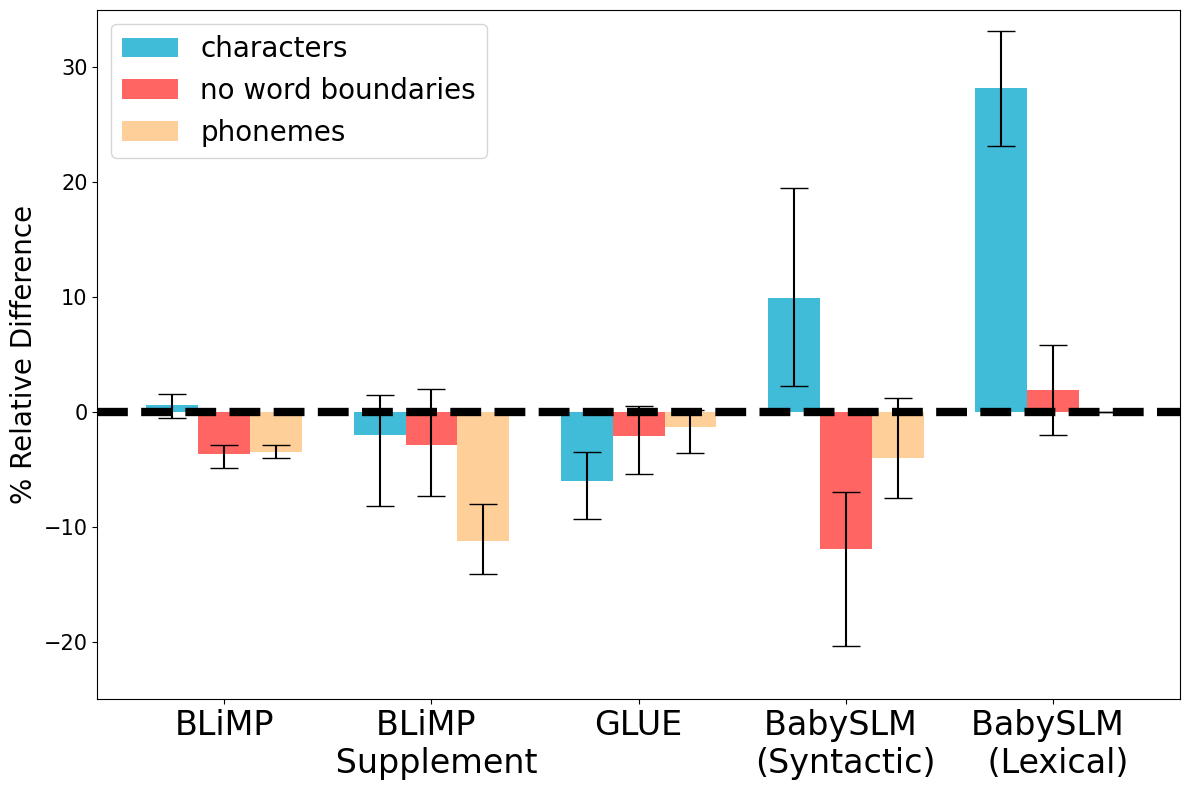
\includegraphics[width=0.9\linewidth]{14Modelling/confidence-int.png}
      \caption{Mean (with Min and Max range) percentage difference achieved on each benchmark's macro score as a result of the three adjustments.}
    \label{fix:14-condition-differences}
\vspace{-4mm}
\end{figure}

For each transformation, we can create four pairs of runs that only differ with respect to that transformation (e.g.\ the four runs with a phonemic transcription and the four runs with orthographic text). For each pair, we calculate the percentage increase in each metric caused by the transformation. In \cref{fix:14-condition-differences} we plot the average of these four percentage differences, allowing us to identify the overall effect of each transformation. We can also use the averaged scores for each subtask within a benchmark (such as the 67 BLiMP subtasks) to assess whether differences are significant for BLiMP, BLiMP Supplement, GLUE and BabySLM (Syntactic) using a paired $t$-test (see \cref{sec:14-significance} for details and $p$-values for each test conducted).

\paragraph{Character Tokenization} We find that character tokenization does not significantly decrease performance on BLiMP or BLiMP Supplement compared to subword tokenization. This validates previous work which found that despite the higher computation costs, character-based language models are just as capable of learning language \citep{al-rfou_character-level_2019, hahn-baroni-2019-tabula}. We do find a significant decrease for GLUE but this may be due to the fact that many of the finetuning examples for GLUE are very long and our model's context size is only 128 tokens, leading to severe truncation. As character-based tokenizers output more tokens for the same sentence than BPE tokenizers, this means that for many GLUE tasks, necessary information is lost.

\paragraph{Word boundary removal} We find that removing word boundaries significantly decreases the BLiMP score, but the decreases for BLiMP Supplement and GLUE are not significant.\footnote{Since there are only 5 tasks for BLiMP Supplement it is difficult to get a $p$-value below 0.05.} In their investigation, \citet{nguyen-2022-word-boundaries} found a decrease of 7-8\% on their own phonemic version of BLiMP when word boundaries were removed, but here we observe only an average decrease of 3.7\%. As they only trained 3-layer LSTMs, it is possible that larger models like ours are required to overcome the loss of word boundaries.

\paragraph{Phonemic Transcription} Finally, we find that using a phonemic transcription instead of the original written text significantly decreases performance on BLiMP and GLUE, although the percentage decreases are small (3.5\% and 1.5\% respectively). It also leads to the largest decrease of 11.3\% for BLiMP Supplement. We discuss a possible explanation for this particular decrease in \cref{sec:14-punctuation}.

\subsection{BabySLM}
\label{sec:14-babyslm}

Unlike the other benchmarks, our best BabySLM score is not achieved by the model trained with the standard orthographic input representation. Instead, the best syntactic score of 94.9 is achieved by the model that uses character-based tokenization (on written text, with word boundaries) and the best lexical score of 89.6 is achieved by the model that uses character-based tokenization for phonemes. It is also worth noting that, to the best of our knowledge, these are the best BabySLM scores to date (see \cref{sec:14-babyslmcomparison} for a detailed comparison).

Examining the effect of each condition, we find that using a phonemic transcription on average reduces the syntactic score by 4.0\%, which is in line with the other benchmarks discussed above. Unlike the other benchmarks, the character tokenization condition \textbf{always leads to an improvement} for both BabySLM scores: an average increase of 9.9\% for the syntactic score and 23.9\% for the lexical score. The sentences used for the syntactic test are all very short compared to the BLiMP sentences (4 words long on average) so a more fine-grained representation may be more useful. For the lexical test, where single words are compared that often only differ by a single phoneme, it seems more appropriate to use a character-based tokenization as the model needs to learn the distributional properties of individual phonemes, which may be lost in subword units. 

The removal of word boundaries has a contrasting effect on the two scores. It reduces the syntactic score by 11.9\% but increases the lexical score by 1.9\%, the only benchmark where removing word boundaries is a positive change. However, the best individual lexical score was achieved by the model that did include word boundaries, suggesting that word boundaries are a helpful signal for a model learning to distinguish words from non-words, possibly because they help separate short sequences of phonemes that appear across word boundaries but not within words. 

%It is also notable that the decrease in the syntactic score removing word boundaries has a much larger effect for the BPE models (a decrease of 18.9 and 11.1 points) than the character-based models (which both decrease by 6.6). 

For the syntactic score, the worst scores are achieved by the models that learn subwords without word boundaries. For these models, the BPE algorithm is essentially acting as an unsupervised word segmentation algorithm learning to split entire sentences into useful units. With a vocabulary size of 16,000, it seems we learn units smaller than words (morpheme-sized units such as ``un'' in \cref{table:results}) but also units that cross word boundaries (such as ``acon'' in \cref{table:results}). The resulting implicit subword boundaries seem to have particular consequences when evaluating the shorter BabySLM sentences. Using the BPE algorithm in this way could be of interest for word segmentation studies. 

\subsection{The Effect of Punctuation}
\label{sec:14-punctuation}

Punctuation is a feature of written text that is rarely included in phonemic transcriptions, as it does not typically change the way that words are pronounced. However, punctuation in written text does carry important meaning about the structure and tone of sentences. In speech, this information is typically conveyed through intonation, stress and rhythm. By simply stripping punctuation in our phonemic transcriptions, we may be removing information that is important for a model's ability to learn and process language. 

In some instances, na\"ively stripping punctuation can even lead to nonsense sentences. This may explain the large dip in performance for BLiMP Supplement, as three of the five subtasks rely on punctuation to simulate question-answer pairs or dialogue, such as:

\vspace{-1mm}
\begin{center}
\begin{verbatim}
A: What did you break?\nB: I broke a bowl.
\end{verbatim}
\end{center}
\vspace{-1mm}

In the example above, the line break, colon and question mark are used to indicate speaker turns and convey the question-answer nature of the prompt. Removing the punctuation leads to a nonsense sentence, especially when read aloud with no pauses or change in tone to indicate the structure:

\vspace{-1mm}
\begin{center}
\textipa{2}~\textvisiblespace~\textipa{w 2 t}~\textvisiblespace~\textipa{d I d}~\textvisiblespace~\textipa{j u:}~\textvisiblespace~\textipa{b}~\textipa{\*r}~\textipa{eI k}~\textvisiblespace~\textipa{b i:}~\textvisiblespace~\textipa{aI}~\textvisiblespace\\\textipa{b~\*r~o~U~k}~\textvisiblespace~\textipa{2}~\textvisiblespace~\textipa{b oU l}~\textvisiblespace
\end{center}
\vspace{-1mm}

Without punctuation, the names ``A'' and ``B'' seem out of place. A model trained on written text can use punctuation to possibly understand that these are names, but a spoken model without punctuation would struggle to process this sentence.

This reliance on punctuation seems to be the leading cause of the drop in performance on BLiMP Supplement. If we remove the three subtasks where an understanding of punctuation is required to process the sentence, the effect of switching to a phonemic representation reduces the drop in performance considerably from 11.3\% to 0.9\%.

\begin{figure}[t]
    \centering
    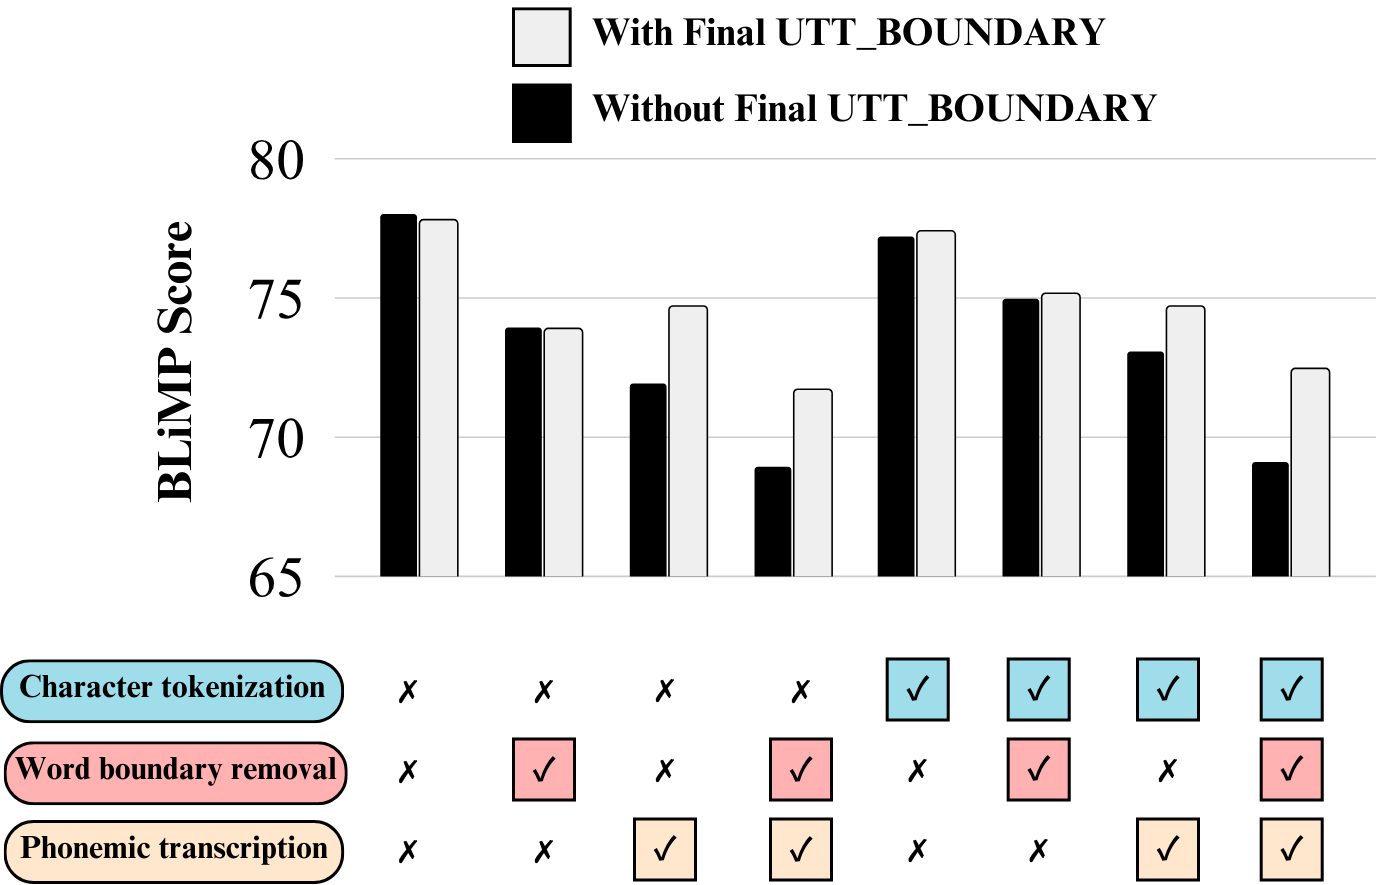
\includegraphics[width=\linewidth]{14Modelling/endofsentencetoken.png}
    \caption{The overall BLiMP scores achieved by GPT-2 in our eight conditions with and without the \texttt{UTT\_BOUNDARY} token (used to separate sentences) included at the end of evaluation instances.}
    \label{fix:14-endofsentencetoken}
\end{figure}

There is another subtle yet crucial consequence of removing punctuation: stripping punctuation at the end of sentences, if not handled correctly, can lead to significant decreases in performance on these benchmarks. This is because without an end-of-sentence marker, certain evaluation examples are no longer valid. In order to mark the end of the sentences without puncutation, we needed to ensure that our dedicated sentence-separation token was added to the end of each evaluation instance. The effect of this adjustment is highlighted in \cref{fix:14-endofsentencetoken}. The increase in BLiMP score for our phonemic models confirms that this change was necessary and highlights the importance of carefully investigating the role of tokenization in the evaluation of large language models. We discuss this effect further in \cref{sec:14-endofsentence}.

\section{Discussion}
\label{sec:14-gap}

In this work, we set out to establish whether modern language model architectures can encode grammatical knowledge and succeed at language understanding tasks when trained with phonemic input representations. By identifying three key transformations, carefully ablating them and evaluating our models on a wide variety of benchmarks, we found that these transformations do lead to decreased performance on standard benchmarks, but that this decrease is not substantial, and the effect of each transformation varies according to the evaluation. Generally, we conclude that language models are capable learners and training with these input representations is completely viable.

In this section, we consider explanations for the difference in performance across the benchmarks and discuss the limitations of phonemic transcriptions and our monolingual approach. Our work also has implications for human acquisition investigations and studies that train models directly from raw audio, which we discuss in \cref{sec:14-further}.

\subsection{The Effect of Input Transformations}

There are many possible explanations for the decrease in performance for BLiMP, BLiMP Supplement and GLUE. In \cref{sec:14-evaluation} and \cref{sec:14-punctuation} we discuss two possibilities; the fact that character tokenization causes more substantial truncation (affecting GLUE) and the fact that phonemic transcriptions do not include punctuation (which particularly affects BLiMP Supplement). Another factor to consider is that although we do not change the GPT-2 architecture or training parameters, the vocabulary size does change, which affects the size of the embedding layer. Character tokenization also leads to reduced exposure to each sentence during training (fewer epochs) because each sentence is represented with more tokens, increasing the number of steps required for each epoch. Furthermore, our initial choice of model parameters may have implicitly favored the standard orthographic input representation given that the language modeling community has been collectively optimizing these architectures to learn representations for written text, not phonemic streams. Just as the BabyLM challenge seeks to find solutions for low-resource language modeling, we may require an equivalent challenge to identify new methods and architectures for a phonemic input representation. 

We also found a different pattern for the BabySLM benchmark, that certain transformations increased performance. In some cases, the transformations were even necessary (the lexical measure requiring a model to be trained on phonemic input). Given that the BabySLM benchmark more closely relates to child-language acquisition with its shorter sentences and vocabulary taken from child-directed speech, this result will be of interest to studies using language models to study acquisition.

\subsection{Limitations and advantages of phonemic transcriptions}
\label{sec:14-phonemeslimitations}

One difficulty in training models from ecological long-form child-centered audio is the lack of corpora available. Papers reporting research on day-long recordings tend not to release the raw data due to privacy concerns (e.g.\ \citet{bergelson-etal-2023,leon-cristia-2024}).
Our method allows us to convert text (which is much more readily available) into a speech representation (phoneme streams), meaning that we could quickly prepare a corpus of 100 million words. 

There are also limitations in our transcription generation process. The fact that phonemes are an abstraction of speech means that we lose key information contained in speech such as prosody, stress and allophonic variation. Using a single accent to generate our phonemes, we also lose inter-speaker variability. Children also learn from non-linguistic cues, multi-modal input and interaction. If anything, it is a striking result that a model trained only on a set of 51 discrete symbols is able to demonstrate grammatical knowledge and perform competitively at downstream linguistic tasks. 

%[Effect of noise: only 51 symbols to choose from for phoneme data, so each carries less information, so an difference in one token would be harder for the language model to get right compared to 115 characters (possibly). With subwords, way more possibility for distinguishing. Maybe move this up to results and do detailed analysis of some examples.]

\subsection{Multi-lingual evaluation}
\label{sec:14-limitations} 

A final important remark is that our experiments are conducted only in English. It is possible that language models trained on phonemic data in other languages would exhibit different trends in downstream performance. Although a multilingual analysis is outside the scope of our paper, we have applied our data processing pipeline to prepare phonemized datasets for 31 of the languages contained in the CHILDES database and hope to release this dataset in the near future.

\section{Conclusion}

Our study explores the effect of training language models using phonemic input representations, which offer both analytical and practical advantages. We develop a pipeline to convert orthographic datasets into a continuous stream of phonemes and leverage this pipeline to train a language model on phoneme streams and evaluate its grammatical and language understanding abilities. Our findings suggest that while phoneme-based input representations result in a slight decrease in model performance on traditional language understanding tasks, it is nonetheless a feasible training paradigm, facilitating future language modeling work, improving phonological interpretability and enhancing speech-based applications.  

%We encourage further research into phonemic input training  to advance our understanding of language models and their applications.

% one of the key advantages of language models—the reliance on orthographic text—and examines how this factor influences their performance. We find that replacing orthographic text with more speech-like representations often leads to a decline in performance across various language undestanding tasks and syntactic abilities. Our work highlight the importance of considering data representation in language acquisition research and offers straightforward preprocessing methods as a step toward more human-like input for language models.]

Our experiments were performed using resources provided by the Cambridge Service for Data Driven Discovery (CSD3) operated by the University of Cambridge Research Computing Service, provided by Dell EMC and Intel using Tier-2 funding from the Engineering and Physical Sciences Research Council (capital grant EP/T022159/1), and DiRAC funding from the Science and Technology Facilities Council. Z\'ebulon Goriely's work is supported by The Cambridge Trust. Richard Diehl Martinez is supported by the Gates Cambridge Trust (grant OPP1144 from the Bill \& Melinda Gates Foundation). Andrew Caines and Paula Buttery are supported by Cambridge University Press \& Assessment. 
Lisa Beinborn's work is partially supported by the Dutch National Science Organisation (NWO) through the VENI program (Vl.Veni.211C.039).

\section{Implementation Details}\label{app:14-implementation_details}

We implement all experiments using the \texttt{PyTorch} framework \citep{paszke-etal-2019-pytorch} and the \texttt{Transformers} library \citep{wolf-etal-2020-transformers}.

\subsection{Hardware Details}

We use a server with one NVIDIA A100 80GB PCIe GPU, 32 CPUs, and 32 GB of RAM for all experiments. Below, we report a subset of the output of the \emph{lscpu} command:

\begin{tcolorbox}[left=5pt,right=5pt,top=5pt,bottom=5pt]
\small
\begin{verbatim}
Architecture:        x86_64
CPU op-mode(s):      32-bit, 64-bit
Address sizes:       46 bits physical, 
                     48 bits virtual
Byte Order:          Little Endian
CPU(s):              32
On-line CPU(s) list: 0-31
Vendor ID:           GenuineIntel
Model name:          Intel(R) Xeon(R)
                     Silver 4210R CPU
                     @ 2.40GHz
CPU family:          6
Model:               85
Thread(s) per core:  1
Core(s) per socket:  1
Socket(s):           8
Stepping:            7
BogoMIPS:            4800.11
\end{verbatim}
\end{tcolorbox}

\subsection{Model Parameters and Training Procedure}

\begin{table}[ht!]
    \centering
    \small
    \begin{tabular}{lc}
    \toprule
         Parameter & Value\\
    \midrule
         Layers & 12 \\
         Heads & 12 \\
         Dropout & 0.1 \\
         Embedding Size & 768 \\
         Inner Size & 3072 \\
         Max Example Length & 128 \\
         Learning Rate & 0.001 \\
         Optimizer & AdamW \\
         Scheduler Type & Linear\\
         Max Steps & 400,000 \\
         Warm-up Steps & 90,000\\
         Per Device Batch Size & 32 \\
    \bottomrule
    \end{tabular}
    \caption{Hyperparameter settings for training the GPT-2 architecture. Vocabulary size varies according to the tokenizer used, but all other parameters are constant across experiments. Where values are not reported, they may be assumed to be default values.}
    \label{table:baseline_hyperparams}
\end{table}

We describe the model and training parameters in \cref{table:baseline_hyperparams}. The model parameters were chosen to match those of the Pythia-170M model from the Pythia suite \citep{biderman2023pythia}. The model has 85M non-embedding parameters and is also equivalent in size to GPT-Neo 125M and OPT-125M. The Pythia models use the GPTNeoX architecture which is slightly different to GPT-2. In initial experiments, we found that GPT-2 performed better on the benchmarks across all eight of our conditions. 

Data is prepared into batches by first tokenizing the entire dataset, combining all tokens into one long vector, and then splitting the vector into chunks of 128 tokens. Only the very last example is padded, if required. At each step during training, random chunks are selected and combined into batches. 

Checkpoints are taken every 50,000 steps during training. At each checkpoint, the perplexity is evaluated on the held-back evaluation set, and at the end of training the checkpoint with the lowest perplexity is returned as the best model. 

\section{Evaluation Details}

\subsection{Significance Tests}
\label{sec:14-significance}

\begin{table*}[t]
    \centering
    \small
    \begin{tabular}{l|cccc}
     & BLiMP&BLiMP Supplement & GLUE & BabySLM (Syntactic) \\
\hline
orthographic vs.\ phonemic & \textbf{0.0001} & 0.0780 & \textbf{0.0149} & 0.1884 \\
word boundaries vs.\ no word boundaries & \textbf{0.0000} & 0.1831 & 0.0813 & \textbf{0.0118} \\
character tokenization vs.\ subword tokenization & 0.5069 & 0.4832 & \textbf{0.0010} & 0.1500 \\
    \end{tabular}
    \caption{$p$-values from the paired student t-tests for each experiment. Significant results are given in \textbf{bold} using an alpha level of 0.05.}
    \label{tab:14-pvalues}
\end{table*}


It is difficult to determine whether the results for a given benchmark are significant given that we only train a single run for each of the eight conditions. Instead, we calculate the significance of a particular transformation by comparing the scores for each subtask of a benchmark. We average the scores achieved by the four models with a transformation applied and average the scores achieved by the four models without the transformation applied, giving us paired results for each subtask. We then use a paired student $t$-test to assess the significance of the transformation. We give the $p$-values for our significance tests in \cref{tab:14-pvalues}.

Note that there are 67 subtasks for BLiMP, 5 for BLiMP Supplement, 9 for GLUE and 9 for BabySLM (Syntactic). With only 5 pairs for BLiMP Supplement, 
%it is difficult to beat the significance level of 0.05.
the test is under-powered and low $p$-values are unlikely. There are no subtasks for BabySLM (Lexical) so significance cannot be computed in the same way. 


\subsection{The Effect of End-of-Sentence Tokens}
\label{sec:14-endofsentence}

By default, our tokenizers add a special start-of-sentence token \texttt{UTT\_BOUNDARY} to all sentences. This corresponds to the \texttt{<s>} token often used by tokenizers to help transformers with sentence-level processing, and also represents utterance boundaries, which unlike word boundaries are a clear cue present in speech and often included in word segmentation studies \citep{feliciano-de-faria-2019-utterance-boundaries}. 

Since sentences are collated together during training, this means that these tokens also appear at the end of every sentence, implicitly acting as end-of-sentence tokens. As a result, the model may use them to represent sentence-level information (especially given that these models are auto-regressive). However, in most evaluation tasks, sentences are presented individually (with padding) and so by default the tokenizer does not add this token to the end of sentences. 

\begin{table*}[t]
    \centering
    \small
    \begin{tabular}{rcc}
        \toprule
        & Grammatical & Ungrammatical \\
        \midrule
       Original & Patrick revealed what a lot of men wore. & Patrick revealed that a lot of men wore. \\
       \midrule
       BPE Text Tokenizer & \makecell{\mybox{<s>}~~\mybox{\textvisiblespace patrick}~~\mybox{\textvisiblespace revealed}~ \mybox{\textvisiblespace what}\vspace{2pt}\\ ~\mybox{\textvisiblespace a}~~\mybox{\textvisiblespace lot}~~\mybox{\textvisiblespace of}~~\mybox{\textvisiblespace men}~~\mybox{\textvisiblespace wore}~~\mybox{\textvisiblespace .}} & \makecell{\mybox{<s>}~~\mybox{\textvisiblespace patrick}~ \mybox{\textvisiblespace revealed}~ \mybox{\textvisiblespace that}\vspace{2pt}\\ ~\mybox{\textvisiblespace a}~~\mybox{\textvisiblespace lot}~~\mybox{\textvisiblespace of}~~\mybox{\textvisiblespace men}~~\mybox{\textvisiblespace wore}~~\mybox{\textvisiblespace .}} \\
       \midrule
       BPE Phoneme Tokenizer & \makecell{ \mybox{<s>}~~\mybox{\textvisiblespace \textipa{p\ae t\*rIk}}~~\mybox{\textvisiblespace \textipa{\*rIvi:ld}}~~\mybox{\textvisiblespace \textipa{w2t}}\vspace{2pt}\\~~\mybox{\textvisiblespace \textipa{2}}~~\mybox{\textvisiblespace\textipa{lAt}} ~~\mybox{\textvisiblespace \textipa{2v}}~~\mybox{\textvisiblespace \textipa{mEn}}~~\mybox{\textvisiblespace \textipa{wO\*r}}} & \makecell{ \mybox{<s>}~~\mybox{\textvisiblespace \textipa{p\ae t\*rIk}}~~\mybox{\textvisiblespace \textipa{\*rIvi:ld}}~~\mybox{\textvisiblespace \textipa{T\ae t}}\vspace{2pt}\\~~\mybox{\textvisiblespace \textipa{2}}~~\mybox{\textvisiblespace\textipa{lAt}} ~~\mybox{\textvisiblespace \textipa{2v}}~~\mybox{\textvisiblespace \textipa{mEn}}~~\mybox{\textvisiblespace \textipa{wO\*r}}} \\
       \bottomrule
    \end{tabular}
    \caption{An example sentence pair from the \texttt{wh\_vs\_that\_with\_gap} subtask in BLiMP and the outputted tokens from our two tokenizers that use subwords but do not remove word boundaries. The `\textvisiblespace ' character denotes word boundaries and the `<s>' token represents our \texttt{UTT\_BOUNDARY} token which acts as an utterance boundary and a start-of-sentence token.}
    \label{tab:14-blimpexample}
\end{table*}

This has consequences for zero-shot evaluation tasks where the grammaticality of the sentence depends on the sentence being marked as complete, which is the case for several of the BLiMP subtasks. For instance, one subtask evaluates a model's understanding of filler-gap dependencies by presenting grammatical ``wh''-phrases with ``that''-phrases that are ungrammatical due to a missing dependency. An example is given in \cref{tab:14-blimpexample} along with the tokens produced by two of our tokenizers. Crucially, our phonemic transcriptions do not include punctuation (see \cref{sec:14-punctuation}) and for this task, without an end-of-sentence marker, the ``ungrammatical'' sentence is no longer ungrammatical, as it could just be incomplete.

This means that the subtask remained a valid test for our orthographic models (due to the inclusion of punctuation to mark the end of the sentence), but not the phonemic ones, since for the phonemic models both the ``grammatical'' and ``ungrammatical'' sentences could be considered grammatical. Since this task is not balanced, any preference for the word ``that'' over the ``wh''-words would lead to the model consistently choosing the ``that'' sentences and achieving results below chance (which is 0.5 for all BLiMP tasks).

In our initial experiments we found that the models trained on phonemes achieved scores between 0.06 and 0.14 for this task whereas the orthographic models achieved scores between 0.35 and 0.53. We then added the \texttt{UTT\_BOUNDARY} token to the end of every evaluation instance and found that the phonemic models could then achieve scores between 0.26 and 0.34 (with little change for the orthographic models). These results also held for several other BLiMP tasks with similar constructions. 

We thus decided to ensure that the token was added to the end of every evaluation instance for all benchmarks reported in this paper for two reasons. First, it acts as a necessary end-of-sentence marker to ensure certain tests remain valid for the phonemic models, and second, because the token may encode useful sentence-level information for all models (particularly for GLUE tasks, as only the encoding of the final token is used for predictions).

We present the effect of this decision in \cref{fix:14-endofsentencetoken} which reports the overall BLiMP scores for our eight conditions with and without the inclusion of the \texttt{UTT\_BOUNDARY} token at the end of each evaluation sentence. There is a very large increase for all four phonemic models with little change for the orthographic models, confirming that this was a crucial adjustment.

\subsection{BabySLM Comparison}
\label{sec:14-babyslmcomparison}

In \cref{table:results} we report the BabySLM scores achieved by our models and in \cref{sec:14-babyslm} we mention that these are the highest scores achieved on this benchmark to date. It is worth noting that this is only in comparison to the baseline scores released with the BabySLM benchmark \citep{lavechin}, as at the time of writing no other scores have been published for this benchmark, given how recently it was introduced.

In their study, \citet{lavechin} achieved their highest syntactic score of 70.4 using BabyBERTa \citep{huebner-etal-2021-babyberta} trained on only 5 million words from CHILDES \citep{macwhinney1985child}. All of our models beat this score, with the highest achieving 94.9. BabyBERTa also uses a BPE tokenizer whereas we found that a character-based tokenizer consistently gave better performance (see \cref{sec:14-babyslm}). There is also an architectural difference, BabyBERTa is an autoencoder trained using masked language modeling, whereas our model is autoregressive, using next-token prediction. The LTG-BERT baseline, which is a similarly sized model also trained on 100 million words, only achieves a score of 75.8. The Baby Llama baseline, by comparison, achieves 94.0. It is possible that the autoregressive architecture is much more suited to the syntactic task than the autoencoder architecture of BERT. 

When it comes to the lexical test, the highest score achieved by \citet{lavechin} was 75.4 using a 3-layer LSTM trained on 1.2 million words from the Providence corpus \citep{borschinger-etal-2013-joint} which they converted to a stream of phonemes with no word boundaries using a similar tool to ours. Our highest-scoring model was also trained with character-based tokenization of phonemes, but did include word boundaries, achieving a score of 89.6. Our model without word boundaries got the second-highest score with 87.8.

In both cases, our model is larger (12 layers) and trained on much more data (100 million words) than the BabySLM baselines. Also, our pre-training dataset contains a wider variety of sentences than just the child-directed utterances in CHILDES. We are currently investigating the effect of model size and training size on the BabySLM scores. In initial experiments, we found that even a 6-layer model trained on only 7 million words from CHILDES was able to achieve a lexical score of 82, but this model also only achieved a syntactic score of 70. We hypothesize that lexical-level knowledge can be learned with less data and by smaller models when compared to learning syntactic knowledge, but this research is ongoing.

%The lack of large, high-quality evaluation benchmarks for these languages, however, remains a considerable challenge. 

%Perhaps language models trained on other languages would not show such a gap in performance, perhaps we have just created the best architectures for english orthographic text.

\section{Further Implications}
\label{sec:14-further}

\subsection{Comparing Human Acquisition to Language Model Learning}
\label{sec:14-acquisition}

% Here we could go into the BabyLM challenge as related work that looks into reducing the advantages language models have over humans, say that our work here contributes to the BabyLM challenge, and finally briefly mention the literature regarding 'advantages' and point to our discussion section on audio-based models. 

The capacity of LMs to learn language from text alone has spurred interest in using such models for acquisition and psychology studies, such as comparing model learning trends to child learning behaviour \citep{evanson-etal-2023-language} and using model outputs to predict human reading times \citep{hollenstein-etal-2021-multilingual}.

To push this research further, recent efforts aim to make language modeling more cognitively plausible \citep{beinborn2024cognitive} by reducing the advantages that typical language models have over humans during the learning process \citep{warstadt-2022-artificial}. One approach is to limit and curate the dataset to that which a typical human may be exposed to, such as is done in the BabyLM challenge \citep{warstadt-2023-babylm-findings}. Another approach is to use an input representation that more closely mimics speech rather than written text \citep{dupoux-2018-cognitive}. Finally, we must consider whether the architectures themselves are suitable linguistic theories, given that they were developed for downstream tasks \citep{baroni-2022-proper}.

In this work we contribute to all three approaches by training a language model with streams of phonemes and assess whether the language model architecture used is advantaged or disadvantaged by these changes according to a wide variety of benchmarks. We hope that this leads to further work studying acquisition using phoneme streams as an input representation. However, while streams of phonemes may seem more cognitively plausible than written text, many studies go further than we do and seek to train directly on raw audio.

\subsection{Learning directly from audio}
\label{sec:14-audiomodels}

Our study focused on alternative input representations for text-based language models, but there is also a field of work dedicated to training models directly from raw audio.
%, a completely separate class of input representations.
In recent years, the Zero Resource Speech Challenge has helped pioneer the development of models that learn unsupervised from raw audio \citep{dunbar_self-supervised_2022}. Models such as STELA \citep{schatz2021early, lavechin2022can} use a two-stage approach, learning a discrete symbolic representation by clustering 10ms chunks of audio, then feeding these to a multi-layered LSTM language model.

These models are also used to study acquisition, regarding raw audio as an input representation that is more cognitively plausible than phonemes; a continuous signal full of noise and non-linguistic information that children must learn to filter. Whether adults even use phonemes as a core linguistic representation, and whether children learn phonemic categories before other stages of acquisition both continue to be a matter of debate \citep{kazanina2018phonemes, matusevych2023infant} and the symbolic representations learned by models such as STELA have a duration four times shorter than phonemes, challenging the assumption that phonemic categories are precursors to later stages of acquisition. 

The gap in linguistic performance between text-based models and audio-based models continues to be substantial. \citet{lavechin} developed BabySLM to compare text-based models to speech-based models and highlighted this gap, but further noted that even speech-based models may not always train on plausible input, many often using audiobooks as their training data \citep{Kahn_2020}. When training the STELA model on 1024 hours of ecological long-form child-centered audio compared to 1024 hours of audiobooks, \citet{lavechin} found that the model trained on long-form audio achieved chance-level syntactic and lexical capabilities, highlighting how far we are from producing architectures that can learn from the same signals as human children.

%While language modeling with phonemes may be regarded as more cognitively plausible than training on written text, even sequences of segmented phonemes are an abstraction from the true nature of the input that children receive, consisting of continuous audio streams full of noise and non-linguistic information that children must learn to filter. Whether adults even use phonemes as a core linguistic representation, and whether children learn phonetic categories before other stages of acquisition both continue to be a matter of debate \citep{kazanina2018phonemes, matusevych2023infant}. 

% In recent years, the Zero Resource Speech Challenge has helped pioneer the development of models that learn unsupervised from audio \citep{dunbar_self-supervised_2022}. Models such as STELA \citep{schatz2021early, lavechin2022can} use a two-stage approach, learning a discrete symbolic representation by clustering 10ms chunks of audio, then feeding these to a multi-layered LSTM language model. The symbolic representations learned by the model have a duration four times shorter than phonemes, challenging the assumption that phonetic categories are precursors to later stages of acquisition. 

%\citet{lavechin} developed the BabySLM evaluation metrics to allow text-based LMs to be compared to speech-based LMs, listing text-based models (including models that train on phoneme strings) as equally low in terms of plausibility compared to audio-based models and highlighting a large gap in performance between text-based and audio-based models. They also note that even speech-based models may not always train on plausible input, many often using audiobooks as their training data \citep{kahn2020libri}. When training the STELA model on 1024 hours of ecological long-form child-centered audio compared to 1024 hours of audiobooks, \citet{lavechin} found that the model trained on long-form audio achieved chance-level syntactic and lexical capabilities, highlighting how far we are from producing architectures that can learn from the same signals as human children.

%\subsection{Lingering advantages}

%[Despite us approaching human-like input, sequences of phonemes are still an abstraction from the true nature of input we receive as children and in our day-to-day lives, which in reality is continuous audio, and full of noise and non-linguistic information. Furthermore, phonemes are themselves an abstraction of phones and are learned representations that may even be learned after some initial stages of acquisition, raising questions as to whether they should be used as a primary representation of the input. Arguably we do get to a point where we process audio into streams of phonemes, but that might happen later, and phonemes are also language-dependent.]

%[Some studies do try to learn from true audio input, but data is very limited. Some do show performance (e.g. the audio book one) but even those have advantages, and once removed (using true raw audio from a child's environment) those same models seem to learn nothing. Perhaps we just need more data, as those represent very little, but perhaps we are further than we thought in terms of producing a model that is able to learn language in exactly the same conditions as our amazing brains.]
